% Compilar con: pdflatex Informe_Tecnico_Laboratorio_2_Deep_Learning.tex
% Ejecutar pdflatex dos veces para actualizar el índice y las referencias.
\documentclass[11pt,letterpaper]{article}

\usepackage[utf8]{inputenc}
\usepackage[T1]{fontenc}
\usepackage{lmodern}
\usepackage{microtype}
\usepackage[letterpaper,margin=2.25cm,headheight=15pt]{geometry}
\usepackage{graphicx}
\usepackage{xcolor}
\usepackage{booktabs}
\usepackage{array}
\usepackage{tabularx}
\usepackage{longtable}
\usepackage{multirow}
\usepackage{float}
\usepackage{caption}
\usepackage{subcaption}
\usepackage{amsmath}
\usepackage{amssymb}
\usepackage{enumitem}
\usepackage{fancyhdr}
\usepackage{titlesec}
\usepackage{hyperref}
\usepackage{url}
\usepackage{lastpage}

\definecolor{Navy}{HTML}{102A43}
\definecolor{Blue}{HTML}{176B87}
\definecolor{Teal}{HTML}{2A9D8F}
\definecolor{Cyan}{HTML}{2E86AB}
\definecolor{Gold}{HTML}{E9A23B}
\definecolor{Red}{HTML}{D95D39}
\definecolor{Ink}{HTML}{17324D}
\definecolor{Soft}{HTML}{F1F7FA}
\definecolor{SoftGreen}{HTML}{EAF8F4}
\definecolor{SoftGold}{HTML}{FFF6E2}
\definecolor{Line}{HTML}{D4E2EA}

\hypersetup{
  colorlinks=true,
  linkcolor=Blue,
  urlcolor=Cyan,
  citecolor=Teal,
  pdftitle={Laboratorio 2 - Deep Learning para Series de Tiempo},
  pdfauthor={Jorge Gabriel Palacios Sales, Pablo Daniel Barillas Moreno y Roberto Emiliano Otoniel Camposeco Torres}
}

\pagestyle{fancy}
\fancyhf{}
\fancyhead[L]{\small\color{Navy}\textbf{CC3084 - Data Science}}
\fancyhead[R]{\small\color{Navy}Laboratorio 2}
\fancyfoot[L]{\small Universidad Galileo}
\fancyfoot[R]{\small Página \thepage\ de \pageref{LastPage}}
\renewcommand{\headrulewidth}{0.4pt}
\renewcommand{\footrulewidth}{0.2pt}

\titleformat{\section}
  {\Large\bfseries\color{Navy}}
  {\thesection}{0.7em}{}
  [\vspace{2pt}\color{Line}\titlerule]
\titleformat{\subsection}
  {\large\bfseries\color{Blue}}
  {\thesubsection}{0.65em}{}
\titleformat{\subsubsection}
  {\normalsize\bfseries\color{Teal}}
  {\thesubsubsection}{0.55em}{}

\setlength{\parindent}{0pt}
\setlength{\parskip}{5.5pt}
\setlist[itemize]{leftmargin=1.5em,itemsep=2pt,topsep=3pt}
\setlist[enumerate]{leftmargin=1.7em,itemsep=2pt,topsep=3pt}
\captionsetup{font=small,labelfont=bf}
\graphicspath{{figuras/}}
\renewcommand{\contentsname}{Contenido}
\renewcommand{\listfigurename}{Lista de figuras}
\renewcommand{\listtablename}{Lista de tablas}
\renewcommand{\figurename}{Figura}
\renewcommand{\tablename}{Tabla}

\newcommand{\metric}[1]{\textcolor{Teal}{\textbf{#1}}}
\newcommand{\code}[1]{\texttt{\detokenize{#1}}}
\newcommand{\smallcode}[1]{{\scriptsize\path{#1}}}
\newcommand{\resultbox}[2]{%
  \begin{center}
  \fcolorbox{#1}{Soft}{%
    \begin{minipage}{0.91\textwidth}
    \vspace{5pt}#2\vspace{5pt}
    \end{minipage}}
  \end{center}
}
\newcommand{\warningbox}[1]{%
  \begin{center}
  \fcolorbox{Gold}{SoftGold}{%
    \begin{minipage}{0.91\textwidth}
    \vspace{5pt}\textbf{\color{Navy}Precaución metodológica.} #1\vspace{5pt}
    \end{minipage}}
  \end{center}
}

\begin{document}

\begin{titlepage}
\pagecolor{Navy}
\color{white}
\vspace*{1.0cm}

{\Large\bfseries UNIVERSIDAD GALILEO\par}
\vspace{0.3cm}
{\large Facultad de Ingeniería\par}
{\large Departamento de Ciencias de la Computación\par}

\vfill

{\color{Teal}\rule{\textwidth}{2.5pt}}\par
\vspace{0.7cm}
{\Huge\bfseries Laboratorio 2\par}
\vspace{0.25cm}
{\LARGE Deep Learning para Series de Tiempo\par}
\vspace{0.5cm}
{\Large\bfseries Informe técnico y análisis reproducible\par}
\vspace{0.7cm}
{\color{Teal}\rule{\textwidth}{2.5pt}}\par

\vfill

\begin{tabular}{@{}>{\bfseries}p{4.0cm}p{10.5cm}@{}}
Curso: & CC3084 - Data Science\\[4pt]
Docente: & García Pérez, Lynette\\[4pt]
Sección: & 11\\[4pt]
Integrantes: &
Jorge Gabriel Palacios Sales\\
& Pablo Daniel Barillas Moreno\\
& Roberto Emiliano Otoniel Camposeco Torres\\[4pt]
Fuente: & Base\_Migracion\_2009-2026jun.xlsx\\[4pt]
Período: & Enero de 2009 a junio de 2026\\
\end{tabular}

\vfill
{\large Guatemala, julio de 2026\par}
\end{titlepage}
\nopagecolor
\color{Ink}

\pagenumbering{roman}
\tableofcontents
\newpage
\listoffigures
\listoftables
\newpage
\pagenumbering{arabic}

\section{Resumen ejecutivo}

Este laboratorio estudia si las redes Long Short-Term Memory (LSTM) pueden
pronosticar dos series mensuales de visitantes internacionales y si su
desempeño supera a los modelos tradicionales ajustados en el Laboratorio 1.
Adicionalmente, se utiliza el conjunto de características \textit{catch22}
para comparar siete series desde múltiples perspectivas temporales.

La base contiene 161,036 registros y 210 meses consecutivos, desde enero de
2009 hasta junio de 2026. Para conservar comparabilidad histórica se define
visitante como la suma de \textit{Turista} y \textit{Excursionista}. Las dos
series empleadas para el pronóstico son el total nacional y la frontera
\texttt{01 La Aurora}. Se mantienen los primeros 147 meses como
entrenamiento y los últimos 63 meses como prueba.

Se evaluaron cuatro configuraciones LSTM por serie. Después del tuneo
cronológico, LSTM-1A fue seleccionada para el total nacional y LSTM-2A para
La Aurora. En prueba, la LSTM del total obtuvo RMSE de 137,339, una mejora de
1.58\% respecto a Prophet. Para La Aurora se obtuvo RMSE de 31,020, una
mejora de 26.24\% frente a suavizamiento exponencial simple.

El análisis \textit{catch22} produjo una matriz de siete series por 22
características. El total nacional y América Del Centro fueron el par más
similar, mientras La Aurora fue la serie más atípica. Finalmente, un modelo
LSTM enriquecido con características \textit{catch22} no superó a la LSTM
base: su RMSE fue 42,907. Este resultado muestra que una representación útil
para describir y agrupar series no necesariamente mejora el pronóstico.

\resultbox{Teal}{%
\textbf{Hallazgo central.} Las LSTM superaron a los mejores modelos del
Laboratorio 1 en ambas series. La mejora fue pequeña en el total nacional,
pero sustancial en La Aurora. El uso adicional de \textit{catch22} dentro de
la red no produjo una mejora predictiva.
}

\section{Objetivos}

\subsection{Objetivo general}

Construir, ajustar y evaluar modelos LSTM para dos series mensuales de
visitantes internacionales, comparar sus resultados con métodos
tradicionales y explorar la similitud de todas las series mediante
\textit{catch22}.

\subsection{Objetivos específicos}

\begin{enumerate}
  \item Reproducir las dos series y la partición temporal del Laboratorio 1.
  \item Evaluar al menos dos configuraciones LSTM por cada serie.
  \item Seleccionar hiperparámetros sin utilizar información del test.
  \item Pronosticar los 63 meses reservados y calcular MAE, RMSE, NRMSE y
  sMAPE.
  \item Comparar los ganadores LSTM con Prophet y SES.
  \item Extraer 22 características \textit{catch22} para siete series.
  \item Estandarizar las características y aplicar PCA, clustering, mapas de
  calor, correlaciones y distancias.
  \item Interpretar los grupos, similitudes y comportamientos atípicos.
  \item Construir una LSTM enriquecida con características
  \textit{catch22} y contrastarla con la LSTM base.
\end{enumerate}

\section{Descripción y preparación de los datos}

\subsection{Fuente y estructura}

La hoja \texttt{Datos} se encuentra en formato largo. Cada fila representa
una combinación de año, mes, vía, frontera, país o agrupación, región y tipo
de viajero. La columna cuantitativa \texttt{Viajero} indica el número de
personas correspondiente a esa combinación.

\begin{table}[H]
\centering
\caption{Controles generales de la base}
\begin{tabular}{lr}
\toprule
\textbf{Indicador} & \textbf{Resultado}\\
\midrule
Registros & 161,036\\
Meses únicos & 210\\
Fecha inicial & Enero de 2009\\
Fecha final & Junio de 2026\\
Faltantes en la medida & 0\\
Valores negativos & 0\\
Frecuencia & Mensual\\
\bottomrule
\end{tabular}
\end{table}

\subsection{Definición de visitante}

La base distingue turistas, excursionistas, viajeros y cruceristas. Se
utilizan exclusivamente turistas y excursionistas:

\[
Y_t =
\sum_{i \in \{\text{Turista},\text{Excursionista}\}}
\text{Viajero}_{i,t}.
\]

La categoría \textit{Viajero} queda excluida porque no representa
necesariamente una visita turística y presenta un quiebre metodológico entre
2022 y 2023. Los cruceristas tampoco mantienen cobertura homogénea durante
todo el período.

\subsection{Series seleccionadas}

Para el ejercicio LSTM se utilizan:

\begin{itemize}
  \item \textbf{Total nacional}: suma mensual en todas las fronteras.
  \item \textbf{01 La Aurora}: suma mensual correspondiente a la principal
  frontera aérea.
\end{itemize}

Para el análisis \textit{catch22} se agregan las tres regiones y las tres
fronteras con mayor acumulado:

\begin{itemize}
  \item Regiones: América Del Centro, América Del Norte y Europa.
  \item Fronteras: 01 La Aurora, 07 Valle Nuevo y 09 San Cristóbal.
\end{itemize}

\begin{figure}[H]
\centering
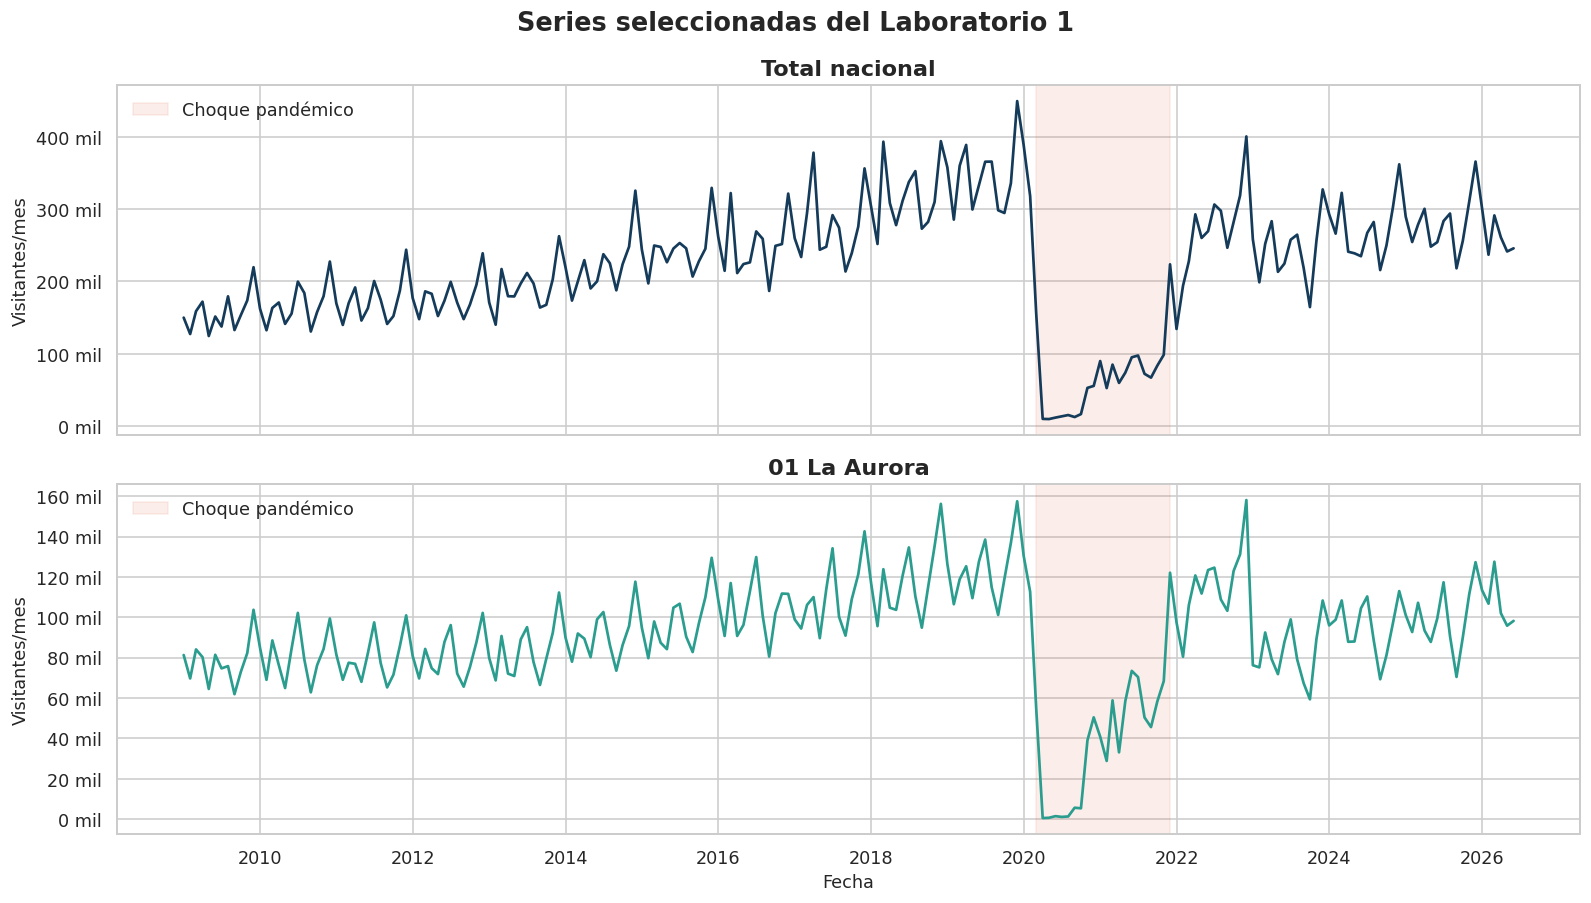
\includegraphics[width=\textwidth]{series_seleccionadas.png}
\caption{Series mensuales utilizadas para el modelado LSTM.}
\label{fig:series}
\end{figure}

Ambas series exhiben crecimiento antes de 2020, estacionalidad anual, un
colapso extraordinario durante la pandemia y una recuperación posterior. La
ruptura de 2020 dificulta el aprendizaje porque no existe un evento
equivalente en los años previos.

\section{Diseño del experimento}

\subsection{Partición externa e interna}

La separación reproduce el Laboratorio 1:

\[
n_{\mathrm{train}}=\lfloor0.70(210)\rfloor=147,
\qquad n_{\mathrm{test}}=63.
\]

El entrenamiento abarca enero de 2009 a marzo de 2021 y la prueba abril de
2021 a junio de 2026. Dentro de los 147 meses se define un tramo interno de
117 meses para ajustar pesos y 30 meses para validar hiperparámetros.

\begin{figure}[H]
\centering
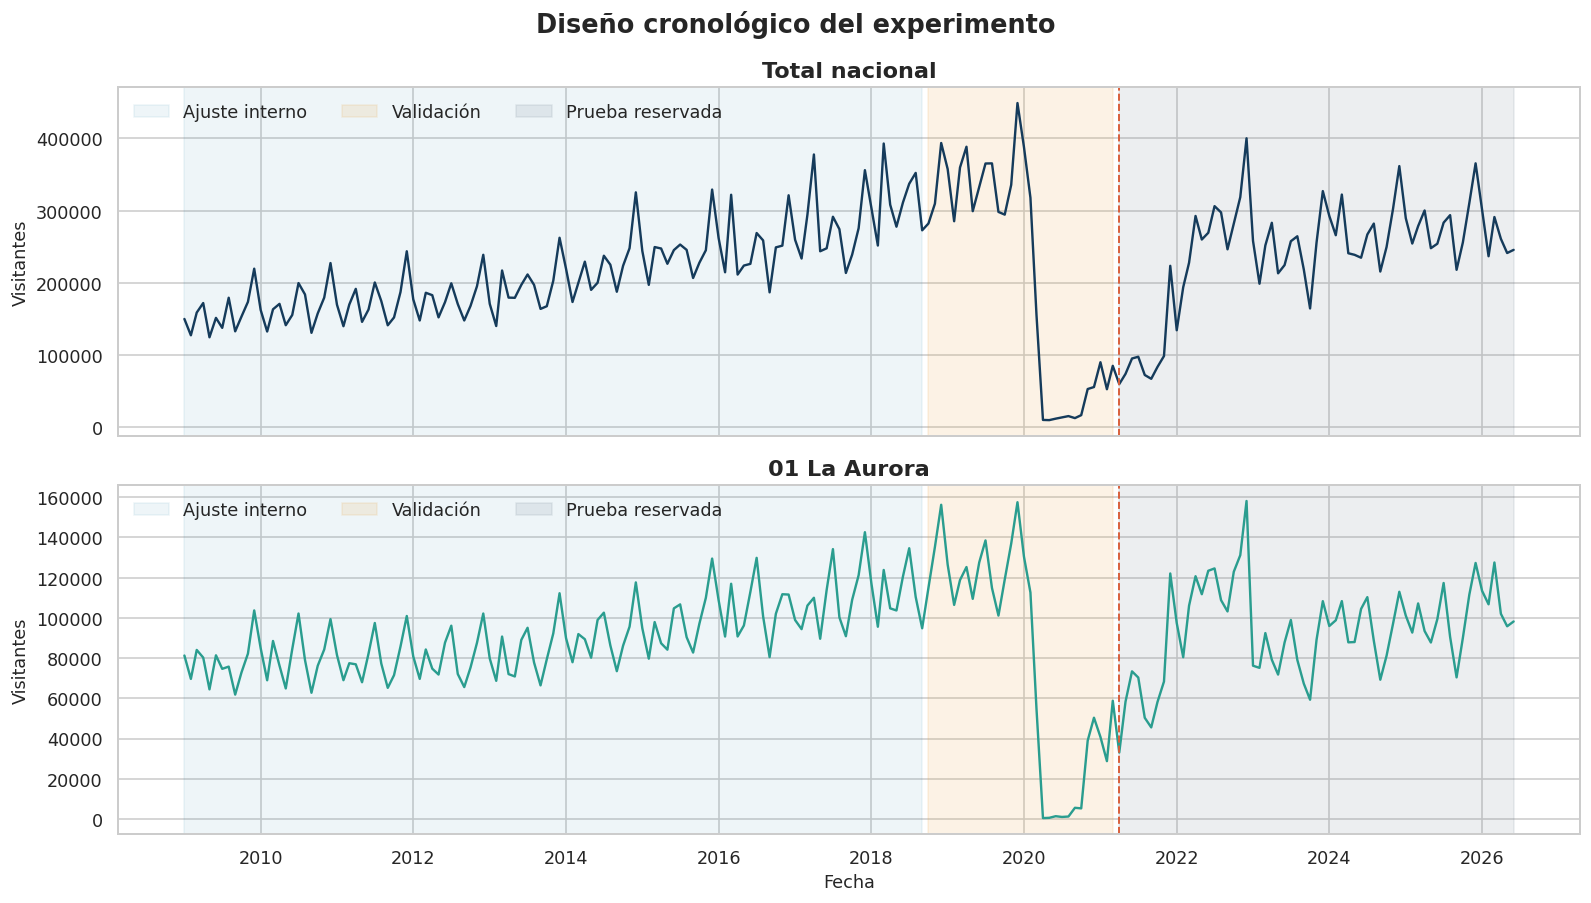
\includegraphics[width=\textwidth]{particion_cronologica.png}
\caption{Partición cronológica de ajuste, validación y prueba.}
\label{fig:split}
\end{figure}

No se barajan las fechas. El escalador Min-Max se ajusta solo con el tramo
interno de entrenamiento durante el tuneo y con los 147 meses completos
durante el reentrenamiento final. El test no se utiliza para seleccionar
arquitecturas, épocas o parámetros.

\subsection{Ventanas supervisadas}

Para una ventana de longitud \(w\), la entrada y el objetivo son:

\[
\left(y_{t-w},\ldots,y_{t-1}\right)\longrightarrow y_t.
\]

Se evalúan ventanas de 12 y 24 meses. La primera contiene un ciclo anual y la
segunda dos ciclos completos. La predicción final es recursiva: cada valor
pronosticado se incorpora al historial temporal para producir el siguiente.

\section{Fundamento del modelo LSTM}

\subsection{Motivación}

Las redes recurrentes procesan datos ordenados y mantienen un estado interno.
Una LSTM agrega puertas que regulan qué información debe conservarse,
actualizarse u olvidarse. Esto reduce el problema de gradientes que se
desvanecen en secuencias largas.

\subsection{Ecuaciones}

Para la entrada \(x_t\), el estado oculto previo \(h_{t-1}\) y la memoria
\(c_{t-1}\), la celda utilizada calcula:

\begin{align}
f_t &= \sigma(W_f[h_{t-1},x_t]+b_f),\\
i_t &= \sigma(W_i[h_{t-1},x_t]+b_i),\\
\widetilde{c}_t &= \tanh(W_g[h_{t-1},x_t]+b_g),\\
c_t &= f_t\odot c_{t-1}+i_t\odot\widetilde{c}_t,\\
o_t &= \sigma(W_o[h_{t-1},x_t]+b_o),\\
h_t &= o_t\odot\tanh(c_t).
\end{align}

La salida final se obtiene mediante una transformación lineal del último
estado oculto. Los pesos se optimizan con Adam. Se aplica regularización L2,
recorte global del gradiente y parada temprana.

\subsection{Implementación reproducible}

La LSTM fue implementada explícitamente en NumPy. La implementación incluye
las cuatro puertas, retropropagación a través del tiempo, una o dos capas,
Adam, semillas deterministas y control de gradiente. Además, se comprobó la
derivada mediante diferencias finitas, con error relativo inferior a
\(10^{-7}\).

\section{Tuneo de hiperparámetros}

\subsection{Espacio de búsqueda}

\begin{table}[H]
\centering
\caption{Configuraciones LSTM evaluadas en cada serie}
\begin{tabular}{llccccc}
\toprule
\textbf{Modelo} & \textbf{Capas} & \textbf{Ventana} &
\textbf{Unidades} & \textbf{Tasa} & \textbf{L2} & \textbf{Lote}\\
\midrule
LSTM-1A & Una & 12 & 8 & 0.010 & 0.0001 & 16\\
LSTM-1B & Una & 24 & 16 & 0.006 & 0.0003 & 16\\
LSTM-2A & Dos & 12 & 12, 6 & 0.006 & 0.0001 & 16\\
LSTM-2B & Dos & 24 & 16, 8 & 0.004 & 0.0003 & 16\\
\bottomrule
\end{tabular}
\end{table}

Se utilizan como máximo 90 épocas, paciencia de 12 épocas y norma máxima del
gradiente de 5. El ganador se define por el menor RMSE de validación en la
escala original de visitantes.

\subsection{Métricas}

\begin{align}
\operatorname{MAE}
&=\frac{1}{n}\sum_{t=1}^{n}|y_t-\widehat{y}_t|,\\
\operatorname{RMSE}
&=\sqrt{\frac{1}{n}\sum_{t=1}^{n}(y_t-\widehat{y}_t)^2},\\
\operatorname{sMAPE}
&=\frac{100}{n}\sum_{t=1}^{n}
\frac{2|y_t-\widehat{y}_t|}
{|y_t|+|\widehat{y}_t|}.
\end{align}

RMSE es el criterio principal porque penaliza con mayor fuerza los errores
grandes. MAE expresa el error mensual típico y sMAPE permite comparar series
de escalas diferentes.

\subsection{Resultados de validación}

\begin{table}[H]
\centering
\caption{Resultados del tuneo interno}
\small
\begin{tabular}{llrrr}
\toprule
\textbf{Serie} & \textbf{Modelo} & \textbf{MAE} &
\textbf{RMSE} & \textbf{sMAPE}\\
\midrule
La Aurora & LSTM-2A & 38,271 & 52,041 & 63.21\%\\
La Aurora & LSTM-1B & 39,500 & 52,843 & 64.22\%\\
La Aurora & LSTM-2B & 46,354 & 55,376 & 71.23\%\\
La Aurora & LSTM-1A & 50,891 & 60,566 & 74.48\%\\
\addlinespace
Total nacional & LSTM-1A & 94,593 & 121,318 & 64.78\%\\
Total nacional & LSTM-1B & 94,530 & 128,869 & 62.60\%\\
Total nacional & LSTM-2B & 106,658 & 134,268 & 68.60\%\\
Total nacional & LSTM-2A & 104,326 & 137,687 & 66.05\%\\
\bottomrule
\end{tabular}
\end{table}

\begin{figure}[H]
\centering
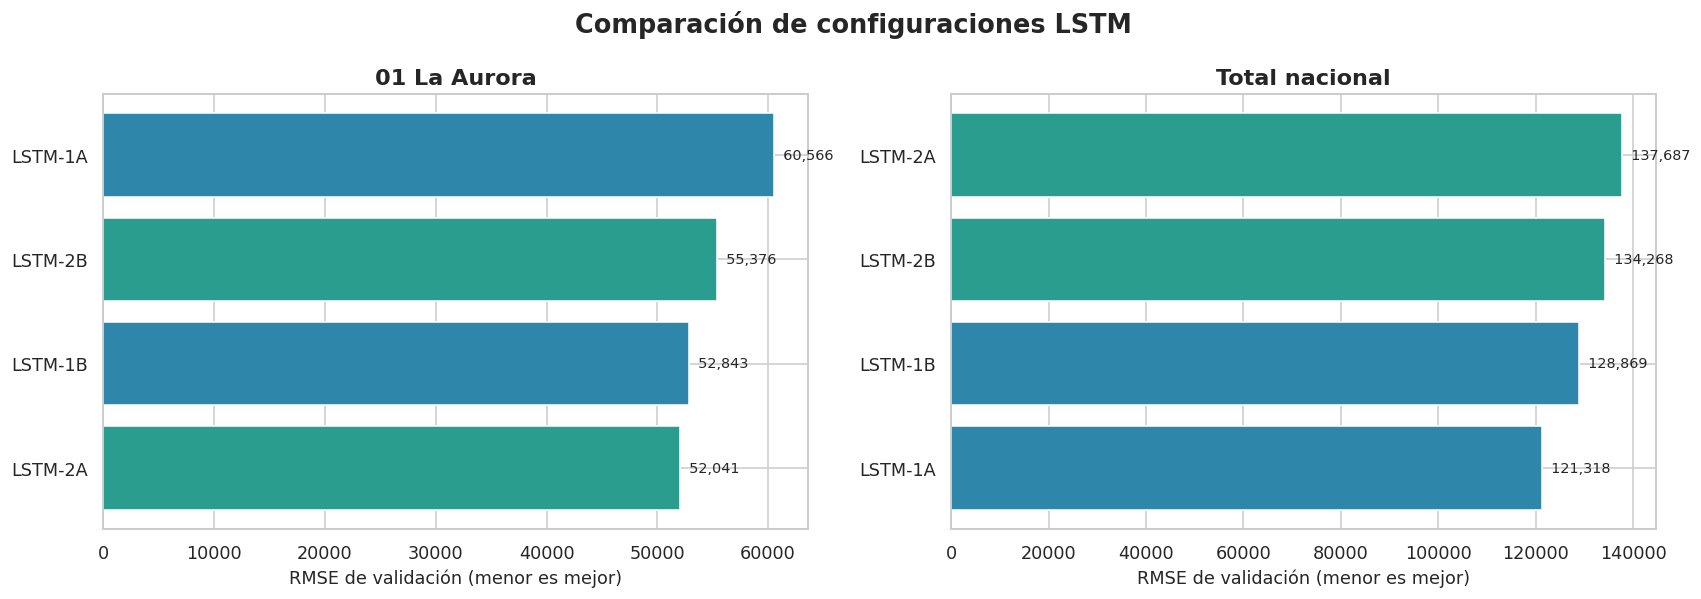
\includegraphics[width=\textwidth]{comparacion_configuraciones.png}
\caption{RMSE de validación de las configuraciones LSTM.}
\label{fig:tuning}
\end{figure}

Los ganadores provisionales son LSTM-2A para La Aurora y LSTM-1A para el
total. Una arquitectura más profunda no garantiza mejor resultado: el total
nacional favorece la red de una sola capa y ocho unidades.

\begin{figure}[H]
\centering
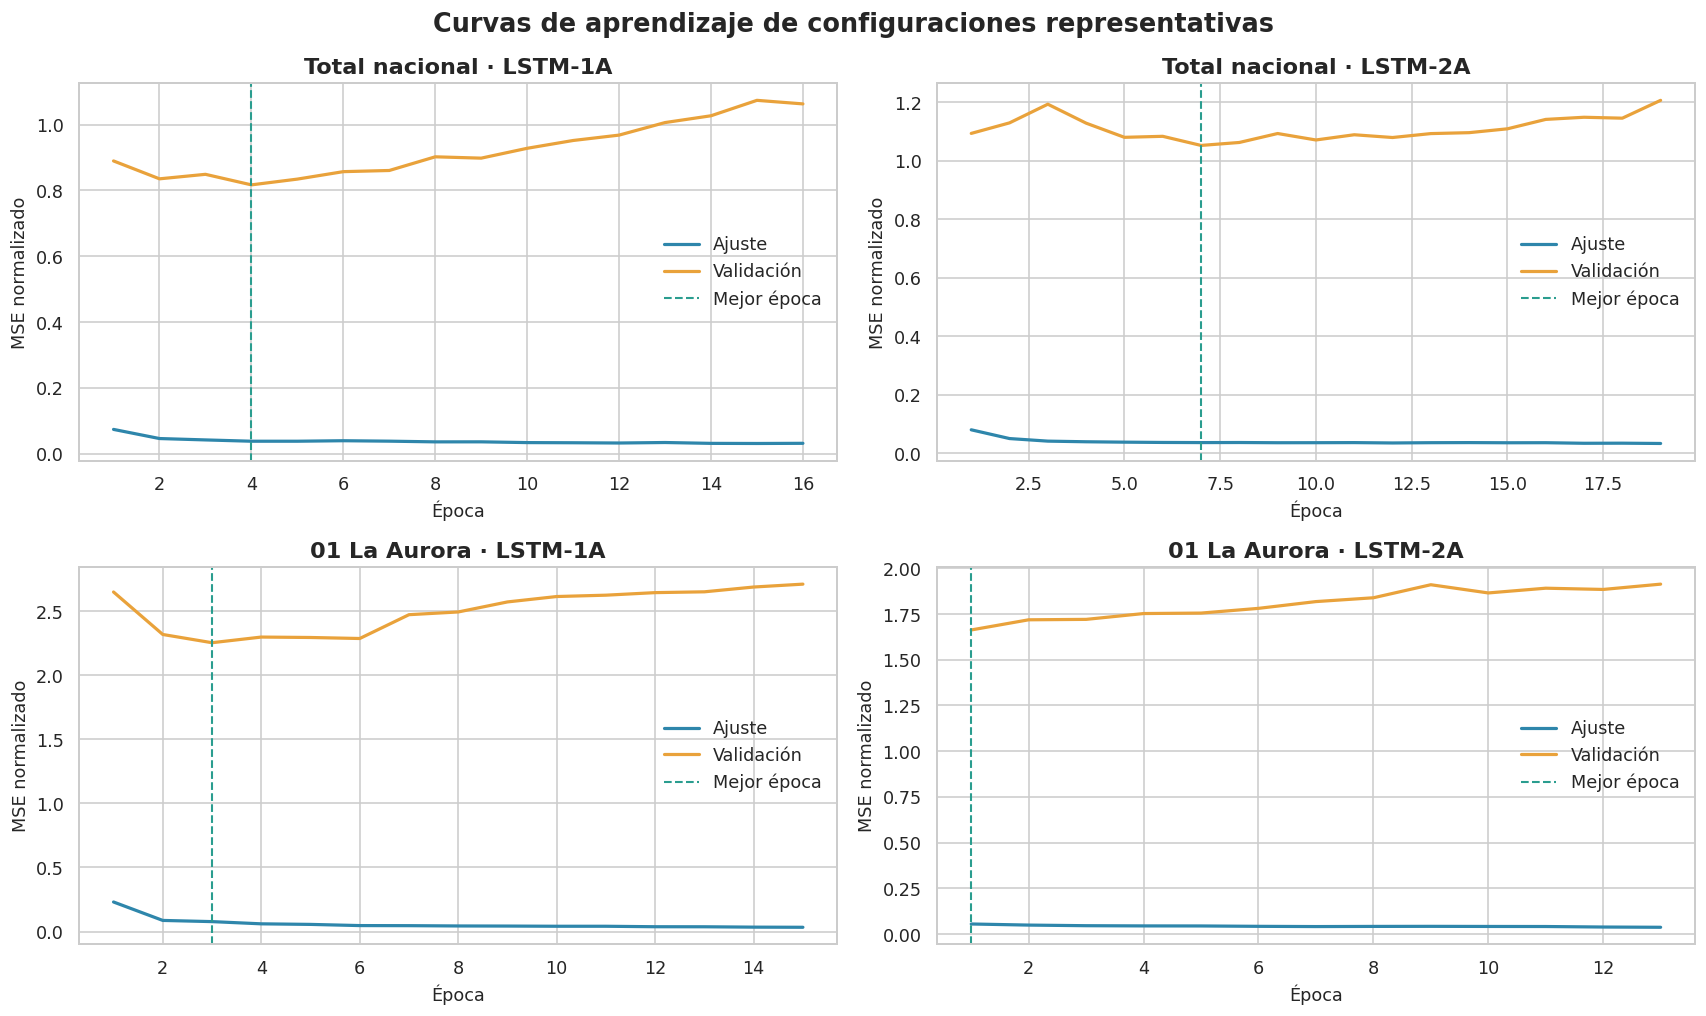
\includegraphics[width=\textwidth]{curvas_aprendizaje.png}
\caption{Curvas de pérdida y época seleccionada.}
\label{fig:curvas}
\end{figure}

La diferencia entre ajuste y validación se explica principalmente por el
cambio de régimen. La validación incluye marzo de 2020 a marzo de 2021. Para
La Aurora, el RMSE durante el choque fue 3.9 veces el error previo; para el
total fue 3.0 veces.

\begin{figure}[H]
\centering
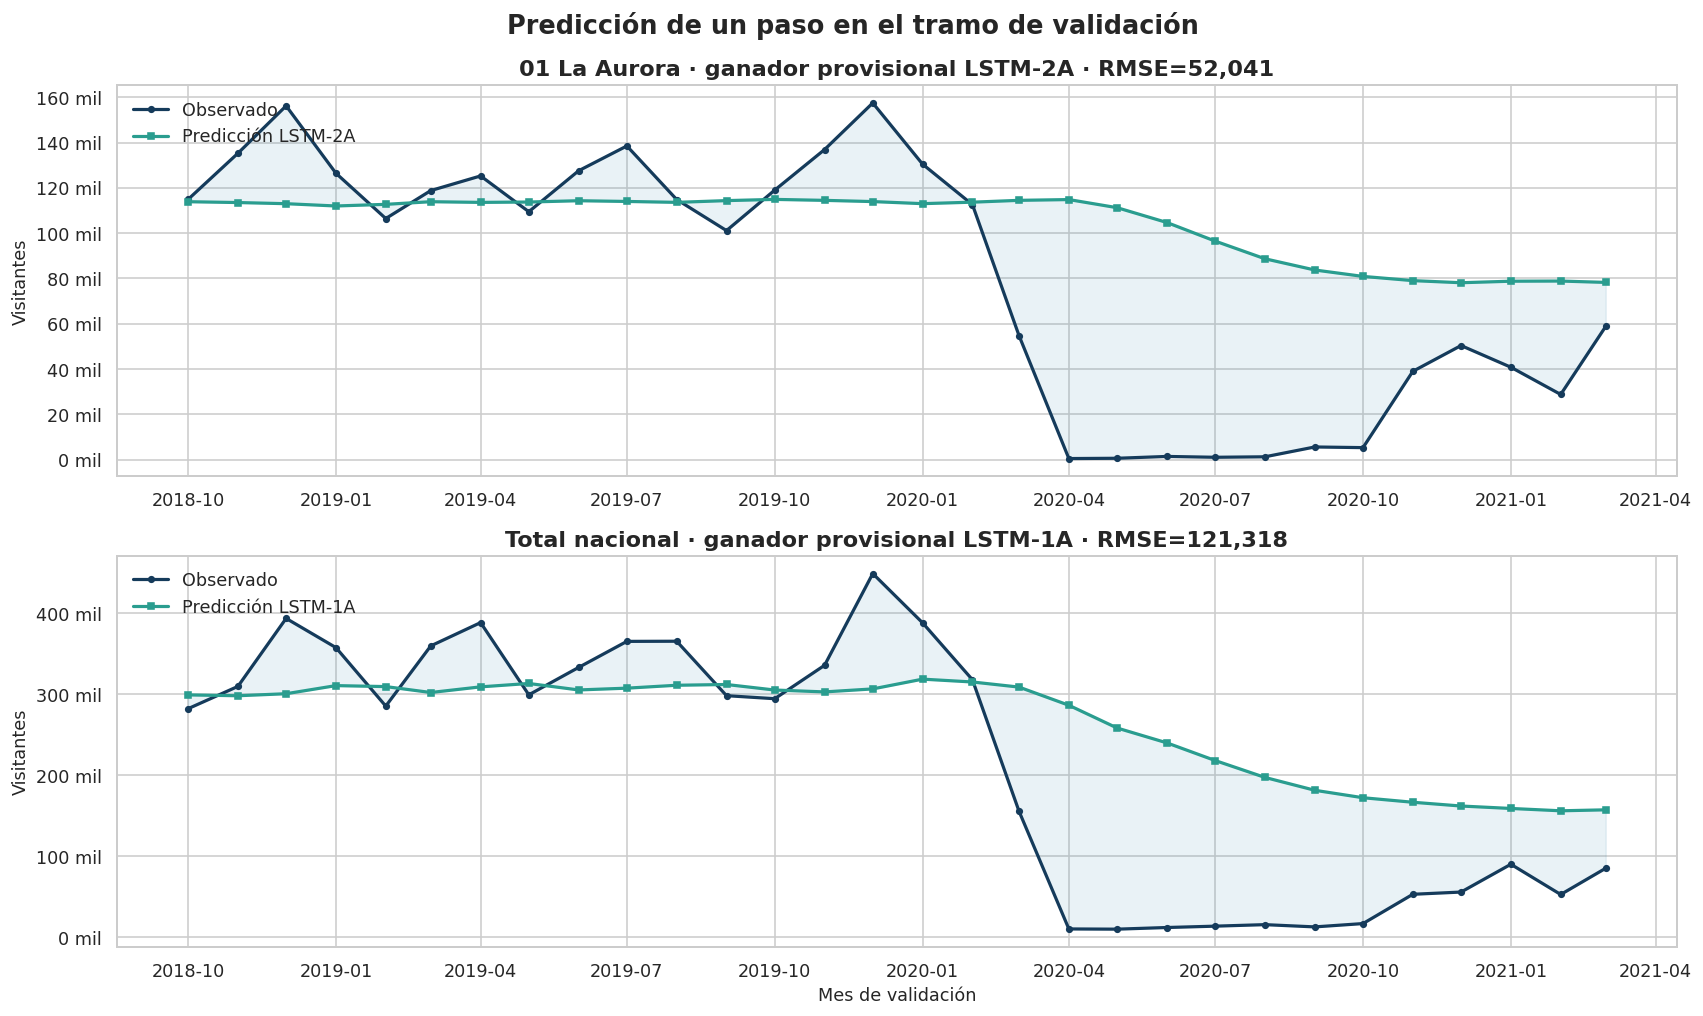
\includegraphics[width=\textwidth]{validacion_predicciones.png}
\caption{Predicción de un paso en el tramo de validación.}
\label{fig:validacion}
\end{figure}

\subsection{Configuraciones descartadas}

La rejilla de la Tabla~5 es reducida a propósito. Se llegó a ese tamaño
después de evaluar redes más grandes y ventanas más largas, cuyos resultados
se documentan aquí porque explican la decisión mejor que un párrafo aislado.

\begin{table}[H]
\centering
\caption{Configuraciones descartadas y su desempeño en validación}
\small
\begin{tabular}{llrrrc}
\toprule
\textbf{Serie} & \textbf{Modelo} & \textbf{RMSE} & \textbf{MAE} &
\textbf{Época} & \textbf{Ventana / unidades}\\
\midrule
Total nacional & LSTM-1X (descartada) & 138,590 & 105,215 & 1/13 & 12 / 64\\
Total nacional & LSTM-2X (descartada) & 119,488 & 98,475 & 32/44 & 36 / 32, 16\\
\addlinespace
La Aurora & LSTM-1X (descartada) & 52,938 & 37,124 & 1/13 & 12 / 64\\
La Aurora & LSTM-2X (descartada) & 58,512 & 48,810 & 17/29 & 36 / 32, 16\\
\bottomrule
\end{tabular}
\end{table}

Los dos casos fallan por caminos distintos. La red de 64 unidades
(LSTM-1X) se detiene en la época 1 con una brecha entre pérdida de ajuste y
de validación de 7.6 veces (0.141 contra 1.066 en el total nacional):
memoriza los 105 ejemplos de ajuste antes de alcanzar a aprender la
estacionalidad. La configuración de ventana 36 sin regularización L2
(LSTM-2X) llega a una brecha de 15.5 veces (0.051 contra 0.792), la mayor de
todas las configuraciones probadas.

\warningbox{En el total nacional, LSTM-2X obtuvo un RMSE de validación
menor que el ganador finalmente seleccionado: 119,488 contra 121,318 de
LSTM-1A, una diferencia de 1.5\%. No se incorporó a la rejilla final ni se
eligió como ganadora por tres razones: (1) la ventana de 36 meses reduce los
ejemplos de ajuste de 105 a 81 y sacrifica los primeros tres años de la
serie; (2) la ventaja no se sostiene en la otra serie, donde LSTM-2X queda
12.4\% por debajo de LSTM-2A en La Aurora (58,512 contra 52,041); y (3) es la
configuración con la mayor brecha entre ajuste y validación, por lo que una
diferencia de 1.5\% en una sola serie no constituye evidencia suficiente. Se
prefirió aplicar un criterio único a ambas series antes que escoger la mejor
cifra de cada tabla por separado.}

\section{Pronóstico definitivo y comparación}

\subsection{Reentrenamiento}

Cada ganador se inicializa nuevamente y se ajusta con los 147 meses
completos. Se utiliza el número de épocas obtenido en la validación: cuatro
para LSTM-1A del total y una para LSTM-2A de La Aurora.

\begin{table}[H]
\centering
\caption{Resultados LSTM sobre el conjunto de prueba}
\begin{tabular}{lrrrr}
\toprule
\textbf{Serie} & \textbf{MAE} & \textbf{RMSE} &
\textbf{NRMSE} & \textbf{sMAPE}\\
\midrule
01 La Aurora & 24,473 & 31,020 & 32.97\% & 28.15\%\\
Total nacional & 123,954 & 137,339 & 56.84\% & 63.35\%\\
\bottomrule
\end{tabular}
\end{table}

\begin{figure}[H]
\centering
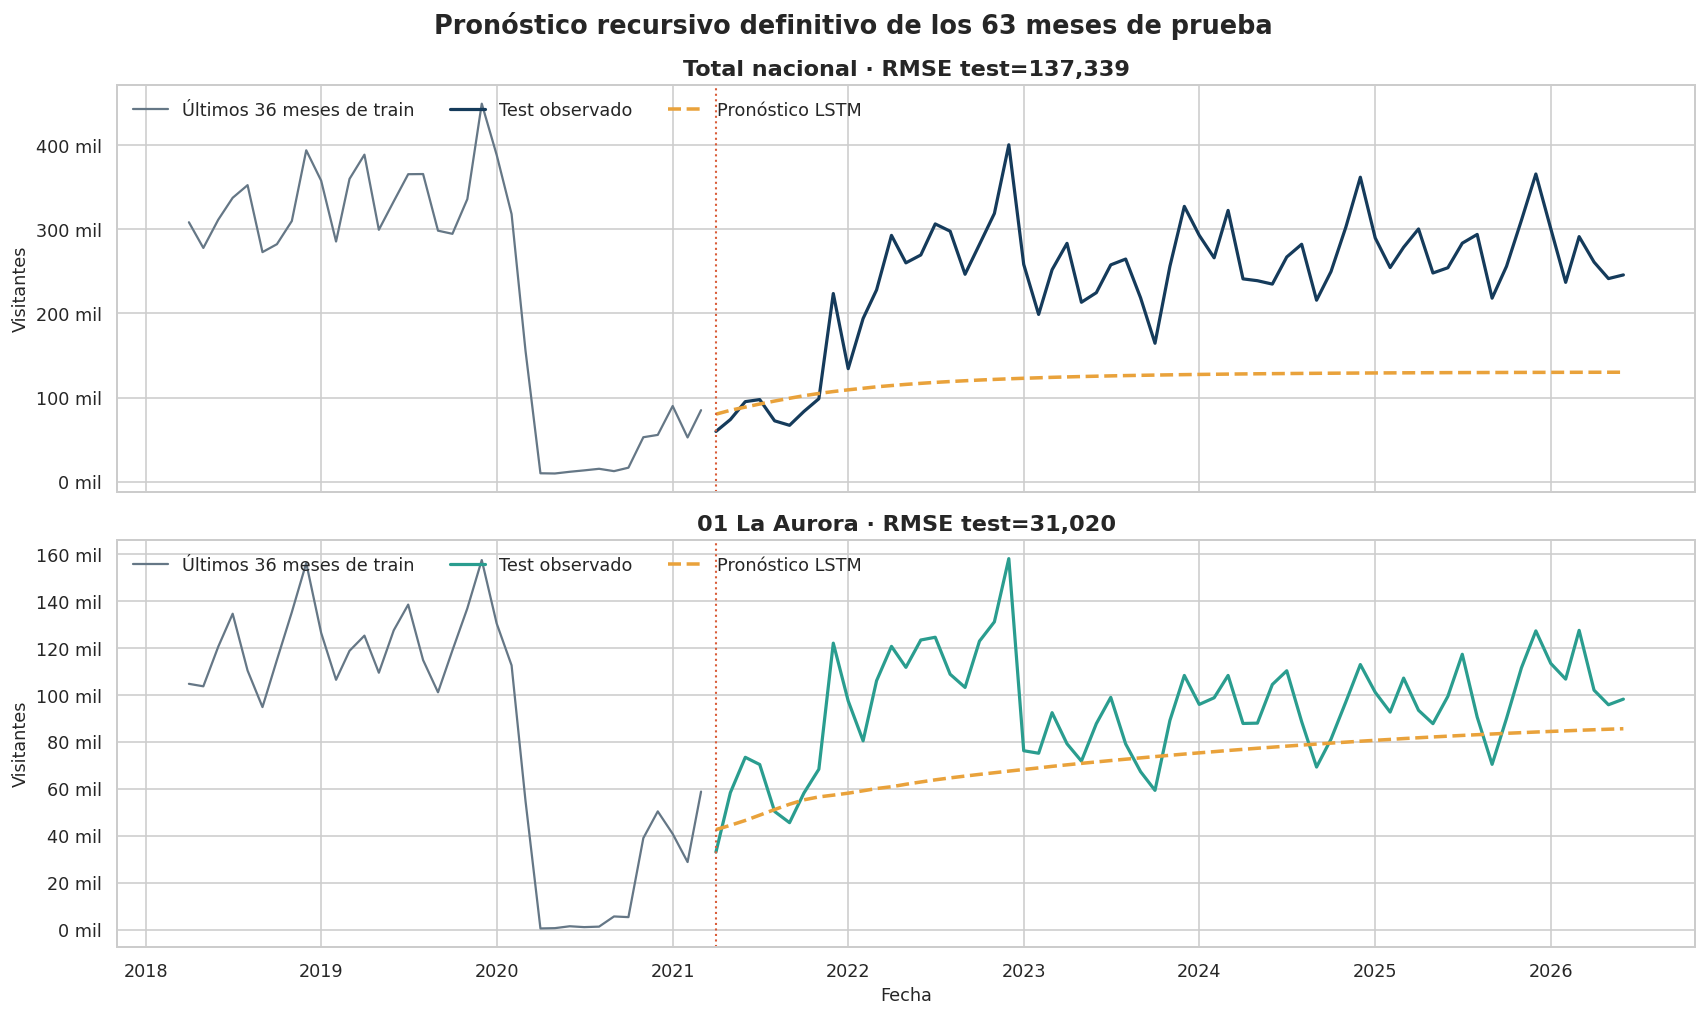
\includegraphics[width=\textwidth]{pronostico_test.png}
\caption{Pronóstico recursivo de abril de 2021 a junio de 2026.}
\label{fig:test}
\end{figure}

La predicción de La Aurora reproduce mejor el nivel general de la
recuperación. En el total nacional, la trayectoria converge a una banda
relativamente estable y no representa completamente los picos mensuales.
Esto explica su NRMSE de 56.84\%.

\subsection{Comparación con modelos tradicionales}

Los valores de referencia provienen del notebook ejecutado del Laboratorio 1.
Prophet había ganado para el total nacional y SES para La Aurora.

\begin{table}[H]
\centering
\caption{LSTM frente al mejor método del Laboratorio 1}
\begin{tabular}{llrrr}
\toprule
\textbf{Serie} & \textbf{Comparación} & \textbf{RMSE LSTM} &
\textbf{RMSE anterior} & \textbf{Mejora}\\
\midrule
01 La Aurora & LSTM-2A vs. SES & 31,020 & 42,053 & 26.24\%\\
Total nacional & LSTM-1A vs. Prophet & 137,339 & 139,549 & 1.58\%\\
\bottomrule
\end{tabular}
\end{table}

\begin{figure}[H]
\centering
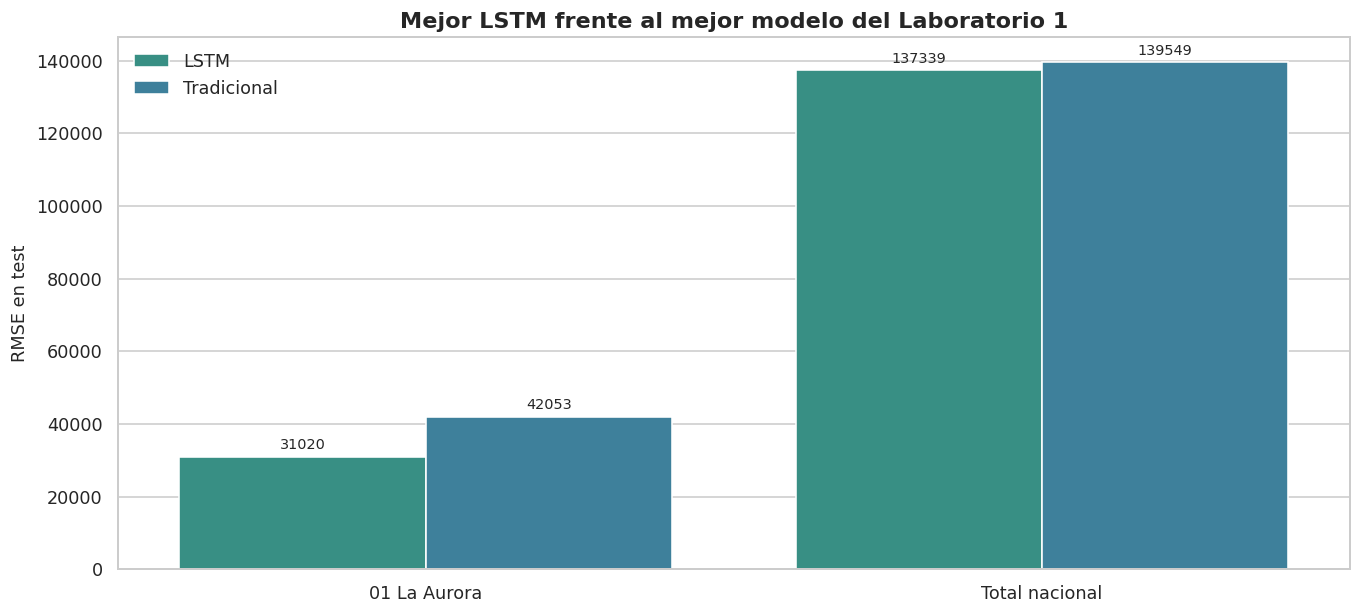
\includegraphics[width=0.92\textwidth]{comparacion_lab1.png}
\caption{Comparación de RMSE en el mismo conjunto de prueba.}
\label{fig:comparacion}
\end{figure}

\resultbox{Teal}{%
\textbf{Respuesta al Ejercicio 1.4.} La LSTM predijo mejor en ambas series
según RMSE. La mejora de La Aurora es clara y alcanza 26.24\%. En el total
nacional la diferencia es de 1.58\%, por lo que debe interpretarse como una
ventaja pequeña y no como superioridad universal.
}

\section{Extracción de características catch22}

\subsection{Concepto}

\textit{catch22} es un conjunto canónico de 22 características seleccionadas
para resumir propiedades de una serie temporal. Incluye medidas relacionadas
con distribución, autocorrelación, periodicidad, información mutua,
comportamiento simbólico, valores atípicos, contenido espectral y
fluctuaciones de largo alcance.

El método permite representar cada serie como un vector de igual longitud.
Así, series con escalas distintas pueden compararse mediante distancias,
proyecciones o agrupamientos.

\subsection{Preprocesamiento}

Cada serie se normaliza primero con media cero y desviación estándar uno. Se
extraen las 22 características mediante \texttt{pycatch22 0.4.5}. La matriz
resultante tiene siete filas y 22 columnas. Luego cada característica se
estandariza entre las siete series:

\[
z_{ij}=\frac{x_{ij}-\overline{x}_{j}}{s_j}.
\]

Esta segunda estandarización evita que una característica con rango amplio
domine PCA, clustering y distancias.

\subsection{Diccionario de características}

\begin{longtable}{p{1.1cm}p{5.8cm}p{8.1cm}}
\caption{Características catch22 utilizadas}\\
\toprule
\textbf{Alias} & \textbf{Nombre oficial} & \textbf{Interpretación breve}\\
\midrule
\endfirsthead
\toprule
\textbf{Alias} & \textbf{Nombre oficial} & \textbf{Interpretación breve}\\
\midrule
\endhead
F01 & \smallcode{DN_HistogramMode_5} & Moda aproximada con cinco intervalos.\\
F02 & \smallcode{DN_HistogramMode_10} & Moda aproximada con diez intervalos.\\
F03 & \smallcode{CO_f1ecac} & Primer cruce de autocorrelación bajo \(1/e\).\\
F04 & \smallcode{CO_FirstMin_ac} & Primer mínimo de autocorrelación.\\
F05 & \smallcode{CO_HistogramAMI_even_2_5} & Información mutua con retardo dos.\\
F06 & \smallcode{CO_trev_1_num} & Asimetría temporal de cambios sucesivos.\\
F07 & \smallcode{MD_hrv_classic_pnn40} & Proporción de cambios consecutivos grandes.\\
F08 & \smallcode{SB_BinaryStats_mean_longstretch1} & Racha más larga sobre la media.\\
F09 & \smallcode{SB_TransitionMatrix_3ac_sumdiagcov} & Persistencia de estados simbólicos.\\
F10 & \smallcode{PD_PeriodicityWang_th0_01} & Longitud del patrón periódico dominante.\\
F11 & \smallcode{CO_Embed2_Dist_tau_d_expfit_meandiff} & Estructura geométrica de retardos.\\
F12 & \smallcode{IN_AutoMutualInfoStats_40_gaussian_fmmi} & Primer mínimo de información mutua.\\
F13 & \smallcode{FC_LocalSimple_mean1_tauresrat} & Dependencia residual tras predictor local.\\
F14 & \smallcode{DN_OutlierInclude_p_001_mdrmd} & Distribución temporal de atípicos positivos.\\
F15 & \smallcode{DN_OutlierInclude_n_001_mdrmd} & Distribución temporal de atípicos negativos.\\
F16 & \smallcode{SP_Summaries_welch_rect_area_5_1} & Potencia relativa de baja frecuencia.\\
F17 & \smallcode{SB_BinaryStats_diff_longstretch0} & Racha de disminuciones consecutivas.\\
F18 & \smallcode{SB_MotifThree_quantile_hh} & Entropía de motivos de tres símbolos.\\
F19 & \smallcode{SC_FluctAnal_2_rsrangefit_50_1_logi_prop_r1} & Escala de fluctuación por rango reescalado.\\
F20 & \smallcode{SC_FluctAnal_2_dfa_50_1_2_logi_prop_r1} & Escala de fluctuación mediante DFA.\\
F21 & \smallcode{SP_Summaries_welch_rect_centroid} & Centroide espectral.\\
F22 & \smallcode{FC_LocalSimple_mean3_stderr} & Error de predictor local de tres puntos.\\
\bottomrule
\end{longtable}

\begin{figure}[H]
\centering
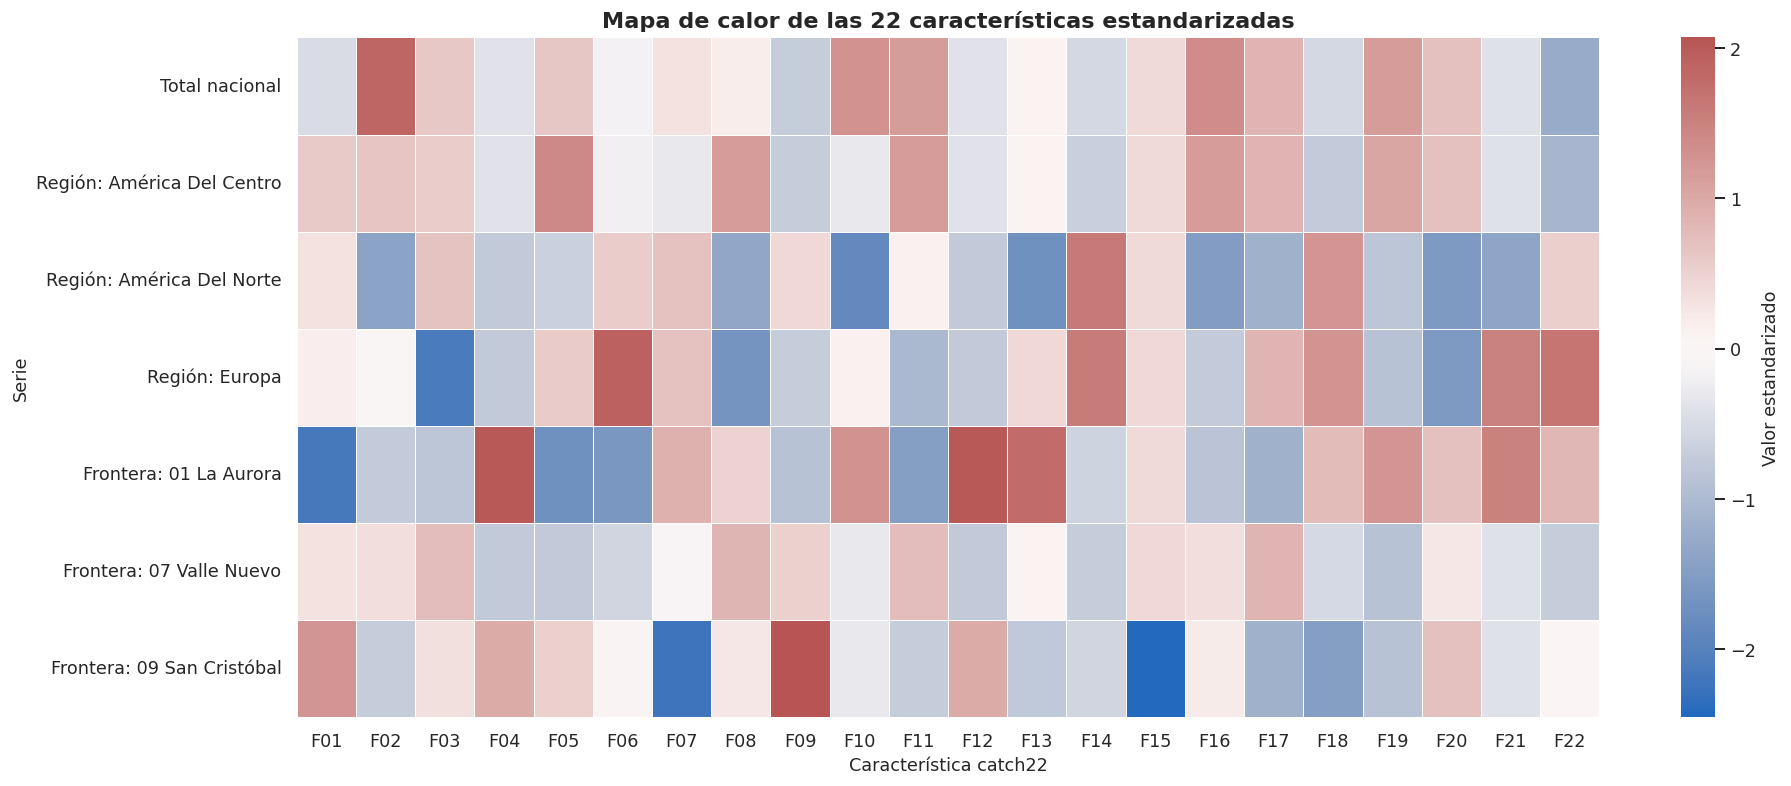
\includegraphics[width=\textwidth]{catch22_heatmap.png}
\caption{Matriz estandarizada de características catch22.}
\label{fig:heatmap}
\end{figure}

\section{Análisis multivariado de catch22}

\subsection{Análisis de Componentes Principales}

PCA transforma las 22 características correlacionadas en ejes ortogonales.
PC1 explica 33.90\% de la variación y PC2 29.14\%; en conjunto representan
63.04\%.

\begin{figure}[H]
\centering
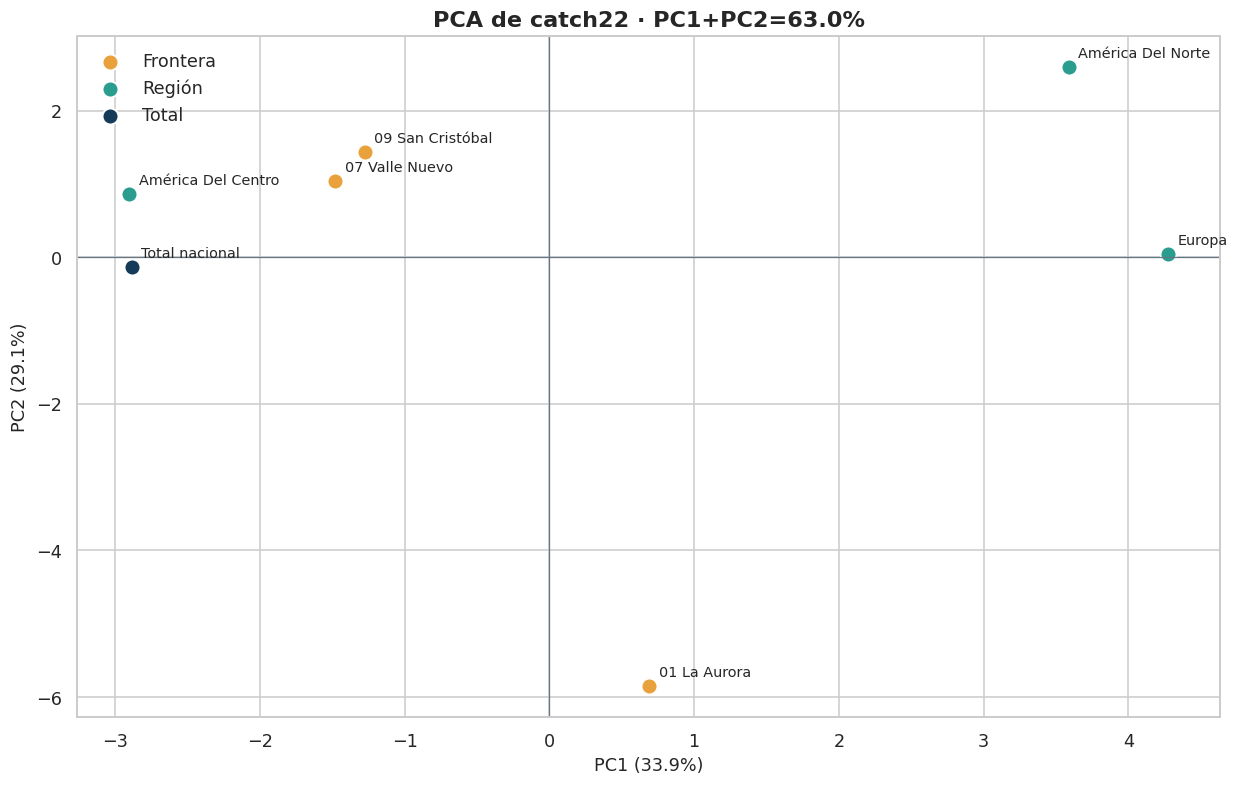
\includegraphics[width=0.88\textwidth]{catch22_pca.png}
\caption{Proyección de las siete series sobre los dos primeros componentes.}
\label{fig:pca}
\end{figure}

El total nacional y América Del Centro aparecen muy próximos. América Del
Norte y Europa ocupan el lado positivo de PC1. La Aurora se separa
principalmente sobre PC2 y constituye el punto más aislado.

Las características con mayor carga conjunta son F01, F20, F13, F14, F22,
F08, F16 y F18. Por tanto, la separación depende de la forma de la
distribución, persistencia, predicción local, atípicos positivos, potencia de
baja frecuencia y estructura simbólica.

\subsection{Clustering jerárquico}

Se compararon dos, tres y cuatro grupos. Los puntajes de silueta fueron 0.207,
0.247 y 0.253, respectivamente. Aunque cuatro grupos produce una diferencia
ligeramente mayor, se seleccionan tres para evitar una fragmentación excesiva
de solo siete observaciones.

\begin{table}[H]
\centering
\caption{Asignación de grupos con clustering Ward}
\begin{tabular}{cl}
\toprule
\textbf{Grupo} & \textbf{Series}\\
\midrule
1 & Total nacional; América Del Centro; Valle Nuevo; San Cristóbal\\
2 & América Del Norte; Europa\\
3 & 01 La Aurora\\
\bottomrule
\end{tabular}
\end{table}

\begin{figure}[H]
\centering
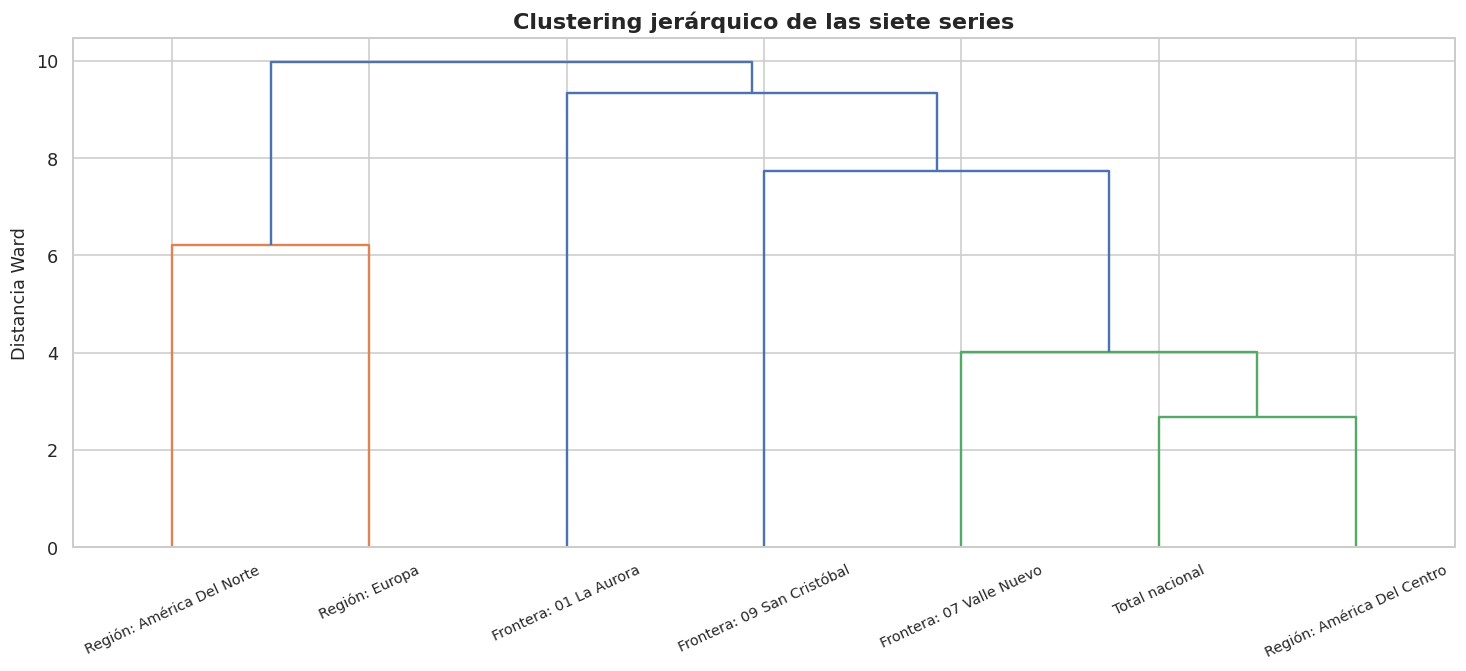
\includegraphics[width=\textwidth]{catch22_dendrograma.png}
\caption{Dendrograma del clustering jerárquico Ward.}
\label{fig:dendrograma}
\end{figure}

El grupo 1 combina el agregado nacional con una región y dos fronteras
terrestres. El grupo 2 contiene dos regiones con perfiles temporales
semejantes. La Aurora forma un grupo propio, lo cual evidencia que las
categorías administrativas no determinan por sí solas la similitud temporal.

\subsection{Distancias entre series}

\begin{figure}[H]
\centering
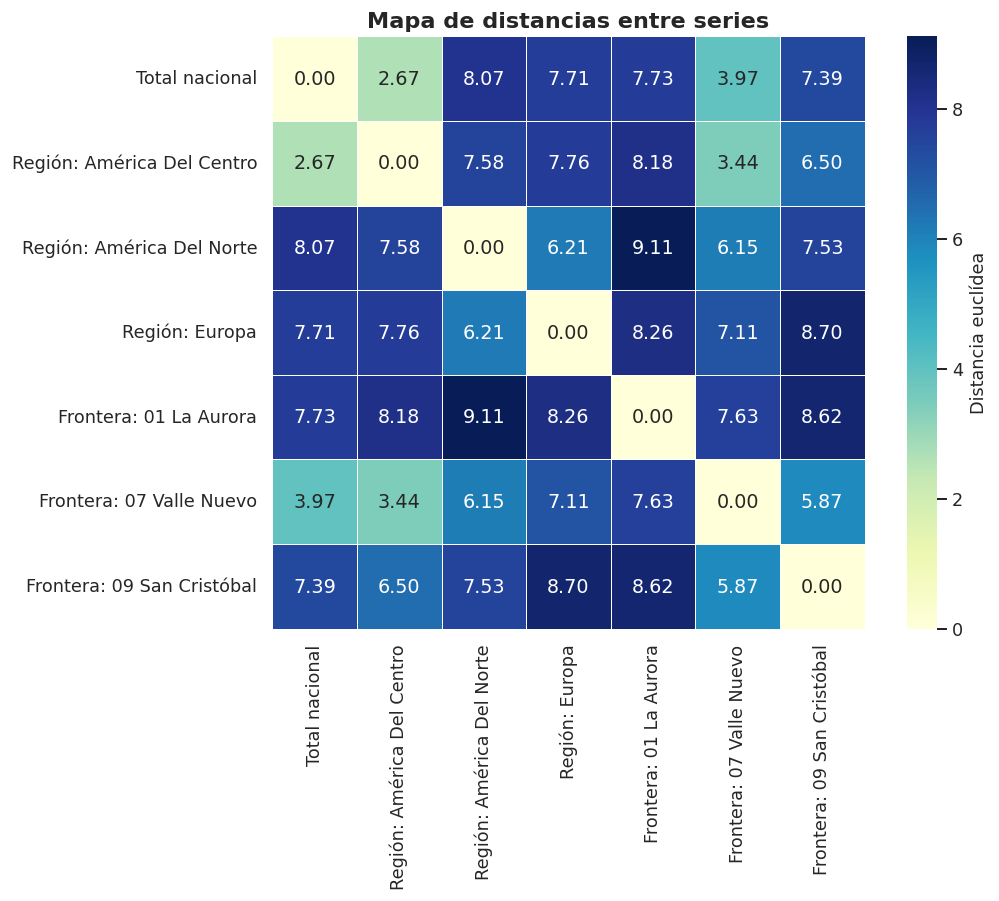
\includegraphics[width=0.82\textwidth]{catch22_distancias.png}
\caption{Distancias euclídeas entre perfiles catch22 estandarizados.}
\label{fig:distancias}
\end{figure}

El par más cercano es total nacional y América Del Centro, con distancia
2.667. Después aparecen América Del Centro con Valle Nuevo (3.440) y total
nacional con Valle Nuevo (3.969). El par más distante es América Del Norte y
La Aurora (9.111).

\subsection{Correlaciones entre características}

\begin{figure}[H]
\centering
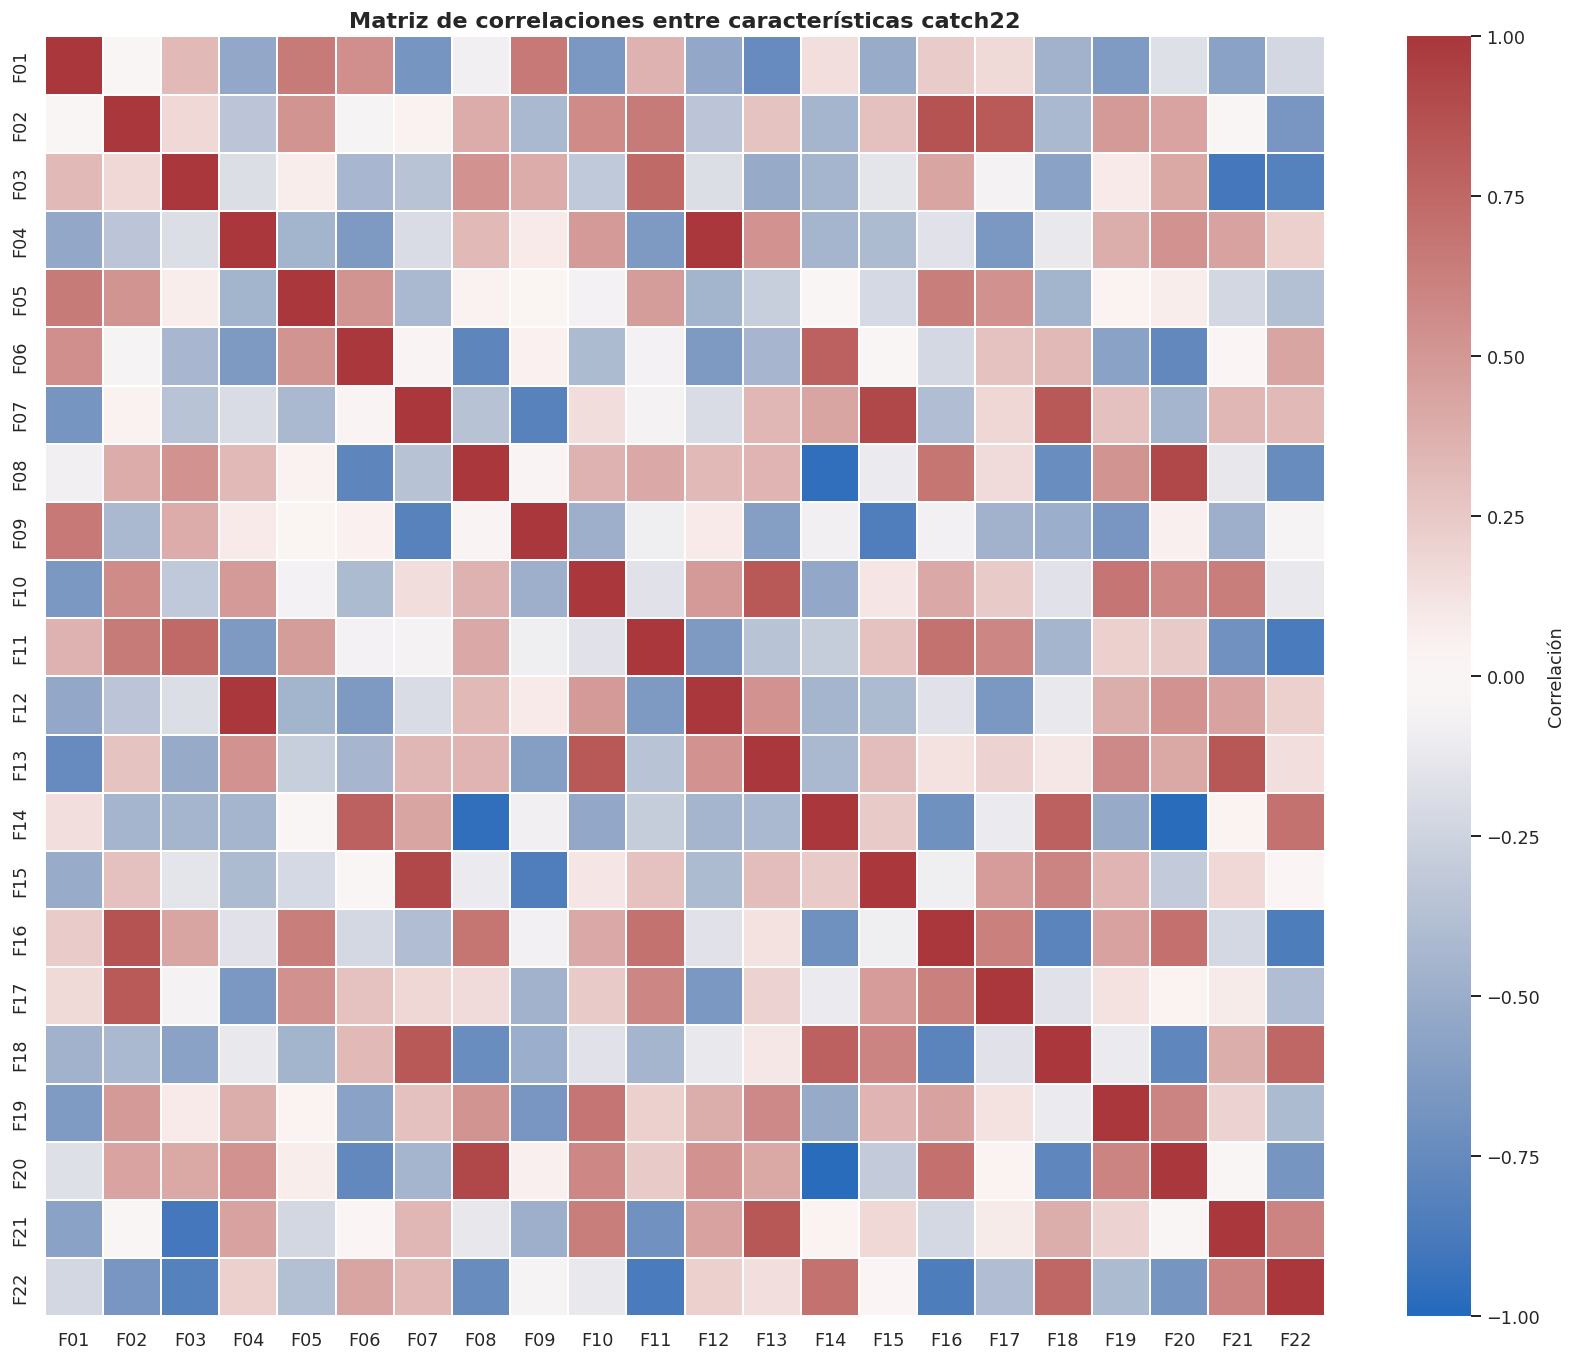
\includegraphics[width=0.88\textwidth]{catch22_correlaciones.png}
\caption{Correlaciones observadas entre las 22 características.}
\label{fig:correlaciones}
\end{figure}

Existen correlaciones altas entre varios descriptores porque algunos resumen
formas relacionadas de persistencia, fluctuación o dependencia. Con solo
siete series, estas correlaciones son exploratorias y no deben generalizarse
como relaciones universales.

\warningbox{El número de variables es mayor que el número de series. PCA,
correlaciones y clustering sirven para explorar esta colección concreta, pero
no constituyen una clasificación definitiva de toda la actividad migratoria.}

\section{Interpretación de los incisos 2.7 a 2.13}

\subsection{Series más similares}

El total nacional y América Del Centro son las más similares según distancia,
PCA y clustering. La explicación contextual es que Centroamérica aporta un
componente importante del total y se relaciona con las principales entradas
terrestres.

\subsection{Características más importantes}

Las cargas de PCA identifican como relevantes la moda de la distribución,
fluctuaciones de largo alcance, capacidad de predicción local, atípicos
positivos, rachas sobre la media, potencia de baja frecuencia y motivos
simbólicos. Estas variables capturan diferencias que una comparación basada
solo en promedios no detectaría.

\subsection{Grupos naturales}

Se observan tres grupos interpretables. El primero refleja la dinámica
centroamericana y terrestre; el segundo reúne Norteamérica y Europa; el
tercero contiene únicamente La Aurora. El puntaje de silueta es modesto, por
lo que los límites entre grupos no son absolutos.

\subsection{Categoría y agrupamiento}

Las series de una misma categoría no siempre se agrupan. Valle Nuevo y San
Cristóbal se acercan al total y a América Del Centro, mientras La Aurora se
separa. Del mismo modo, América Del Centro no queda con las otras dos
regiones. La dinámica observada pesa más que la etiqueta administrativa.

\subsection{Comportamiento atípico}

La Aurora posee la mayor distancia al centroide, 6.053. Su comportamiento
aéreo, el cierre de vuelos, la reapertura y un patrón estacional propio
explican esta posición. Europa y América Del Norte también muestran perfiles
alejados, pero no superan el aislamiento de La Aurora.

\subsection{Consistencia con el análisis anterior}

\begin{itemize}
  \item \textbf{Tendencia}: total y América Del Centro conservan trayectorias
  similares antes de 2020.
  \item \textbf{Estacionalidad}: periodicidad y componentes espectrales
  recuperan diferencias observadas en perfiles mensuales.
  \item \textbf{Volatilidad}: fluctuaciones y error local distinguen series
  con recuperaciones estables de aquellas con cambios bruscos.
  \item \textbf{Pandemia}: atípicos y persistencia representan la duración y
  magnitud desigual del choque.
  \item \textbf{Autocorrelación}: F03, F04 y F12 resumen dependencia temporal
  estudiada previamente mediante ACF.
\end{itemize}

\subsection{Tres descubrimientos adicionales}

\begin{enumerate}
  \item El total se parece más a América Del Centro que a cualquier frontera
  individual, aunque La Aurora sea la frontera de mayor acumulado.
  \item América Del Norte y Europa comparten un perfil temporal multivariado
  pese a sus diferencias de volumen y procedencia.
  \item La categoría frontera no es homogénea: La Aurora se separa, mientras
  Valle Nuevo y San Cristóbal se integran al bloque centroamericano.
\end{enumerate}

\section{Modelo LSTM enriquecido con catch22}

\subsection{Diseño}

Se elige La Aurora porque fue la serie más atípica. El modelo conserva la
arquitectura LSTM-2A y una ventana cruda de 12 meses. Para cada objetivo se
calculan 22 características utilizando únicamente los 36 meses anteriores.
El vector se repite a lo largo de los 12 pasos de entrada:

\[
\mathbf{x}_t=
\left[y_t,f_{1,t}^{(catch22)},\ldots,f_{22,t}^{(catch22)}\right].
\]

La entrada pasa de una a 23 variables por paso. Los descriptores se imputan y
estandarizan solo con el entrenamiento. En el test, se recalculan de forma
recursiva sobre el historial disponible.

\subsection{Resultados}

\begin{table}[H]
\centering
\caption{Comparación del modelo enriquecido en La Aurora}
\begin{tabular}{lrrr}
\toprule
\textbf{Modelo} & \textbf{MAE} & \textbf{RMSE} & \textbf{sMAPE}\\
\midrule
LSTM-2A base & 24,473 & 31,020 & 28.15\%\\
SES & 36,822 & 42,053 & 45.47\%\\
LSTM-2A + catch22 & 34,356 & 42,907 & 43.58\%\\
\bottomrule
\end{tabular}
\end{table}

\begin{figure}[H]
\centering
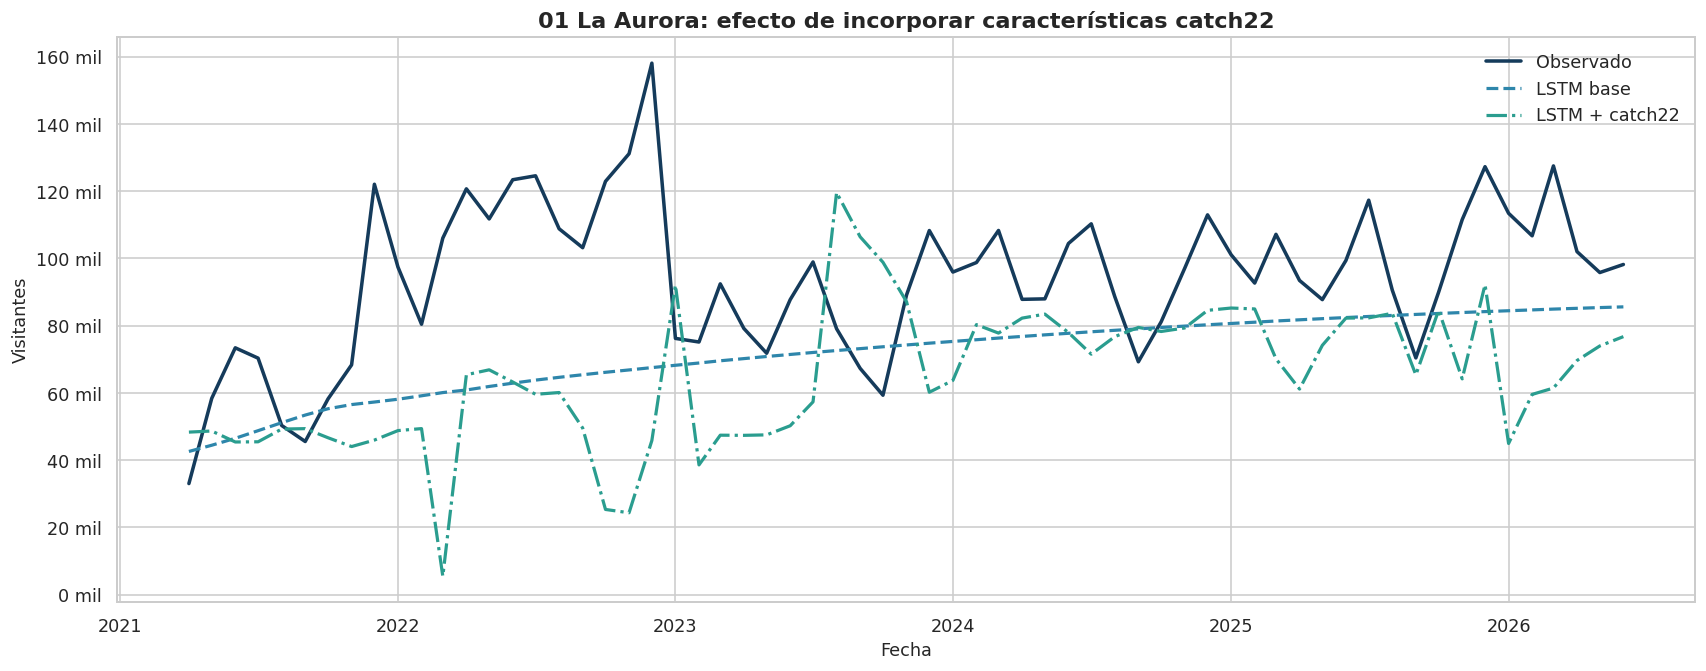
\includegraphics[width=\textwidth]{lstm_catch22.png}
\caption{Predicción base y predicción enriquecida para La Aurora.}
\label{fig:enriquecido}
\end{figure}

El modelo enriquecido empeora el RMSE en aproximadamente 38.32\% respecto a
la LSTM base. También queda ligeramente por debajo de SES. El resultado no
invalida \textit{catch22}: las características fueron eficaces para comparar
series, pero al repetirse en cada paso aumentan la dimensionalidad con pocos
ejemplos y pueden introducir redundancia.

Una arquitectura futura podría procesar la secuencia mediante una LSTM y el
vector \textit{catch22} mediante una rama densa independiente antes de
combinar ambas representaciones.

\section{Conclusiones}

\begin{enumerate}
  \item Se ajustaron ocho candidatos LSTM, cuatro por serie, con tuneo
  cronológico y sin utilizar el test.
  \item LSTM-2A fue la mejor configuración para La Aurora y LSTM-1A para el
  total nacional.
  \item En prueba, las LSTM superaron a los ganadores del Laboratorio 1. La
  mejora fue 26.24\% para La Aurora y 1.58\% para el total.
  \item La matriz \textit{catch22} identificó al total nacional y América Del
  Centro como el par más similar.
  \item La Aurora fue la serie más atípica y formó un grupo propio.
  \item Las categorías administrativas no garantizan comportamientos
  temporales semejantes.
  \item Añadir \textit{catch22} directamente a la entrada LSTM no mejoró la
  predicción. La LSTM base fue más simple y precisa.
\end{enumerate}

\section{Limitaciones y recomendaciones}

\begin{itemize}
  \item El test inicia durante la recuperación pandémica y cubre un horizonte
  largo de 63 meses.
  \item Los modelos no incluyen vuelos, cierres, feriados, tipo de cambio o
  actividad económica.
  \item Solo se estudiaron siete series para el análisis multivariado.
  \item El mejor modelo debe actualizarse conforme se incorporen meses nuevos.
  \item Para uso institucional se recomienda comparar periódicamente LSTM,
  Prophet, suavizamiento y modelos estacionales.
  \item Las predicciones deben acompañarse con intervalos de incertidumbre y
  escenarios cuando se utilicen para planificación.
\end{itemize}

\section{Verificación de cumplimiento}

\begin{longtable}{p{10.8cm}c}
\caption{Correspondencia con las instrucciones del laboratorio}\\
\toprule
\textbf{Requisito} & \textbf{Estado}\\
\midrule
\endfirsthead
\toprule
\textbf{Requisito} & \textbf{Estado}\\
\midrule
\endhead
Dos series y misma partición del Laboratorio 1 & Cumplido\\
Dos configuraciones LSTM por serie & Cumplido\\
Tuneo y selección por validación & Cumplido\\
Pronóstico con el mejor modelo & Cumplido\\
Comparación entre LSTM y contra modelos anteriores & Cumplido\\
Extracción de 22 características para siete series & Cumplido\\
Matriz y estandarización & Cumplido\\
PCA, clustering y mapa de calor & Cumplido\\
Correlaciones y distancias & Cumplido\\
Interpretación de similitudes, grupos y atípicos & Cumplido\\
Tres descubrimientos adicionales & Cumplido\\
LSTM enriquecido con catch22 & Cumplido\\
Código reproducible y ejecutado & Cumplido\\
\bottomrule
\end{longtable}

\section*{Referencias}
\addcontentsline{toc}{section}{Referencias}

\begin{enumerate}[label={[\arabic*]}]
  \item Fulcher, B. D., Little, M. A. y Jones, N. S. (2013).
  \textit{Highly comparative time-series analysis: the empirical structure of
  time series and their methods}. Journal of the Royal Society Interface,
  10, 20130048.
  \item Hochreiter, S. y Schmidhuber, J. (1997).
  \textit{Long Short-Term Memory}. Neural Computation, 9(8), 1735--1780.
  \item Hyndman, R. J. y Athanasopoulos, G.
  \textit{Forecasting: Principles and Practice}.
  \url{https://otexts.com/fpp3/}
  \item Lubba, C. H. et al. (2019).
  \textit{catch22: CAnonical Time-series CHaracteristics}.
  Data Mining and Knowledge Discovery, 33, 1821--1852.
  \item Dynamics and Neural Systems Group.
  \textit{pycatch22}.
  \href{https://github.com/DynamicsAndNeuralSystems/pycatch22}
  {Repositorio oficial de pycatch22}.
  \item Universidad Galileo (2026).
  \textit{Laboratorio 2. Deep Learning. Series de Tiempo}.
\end{enumerate}

\vfill
\resultbox{Blue}{%
\textbf{Nota académica.} La base y los resultados son de uso académico. Las
predicciones no constituyen cifras oficiales ni sustituyen los procesos
institucionales de validación.
}

\end{document}
